\section{Method}
\label{sect:method}

This section presents our unsupervised method for TF design, enabling semi-automated material classification and initial TF specification for intuitive volume exploration.

Fig.~\ref{fig:volume-exploration-pipeline} shows an overview. After organizing the dataset into a volume grid, we apply three steps: dimensionality reduction, clustering, and pivot-based indexing.

\begin{figure*}[htb!]
    \centering
    \caption{Overview of the proposed unsupervised method for transfer function definition and design.}
    \label{fig:volume-exploration-pipeline}
    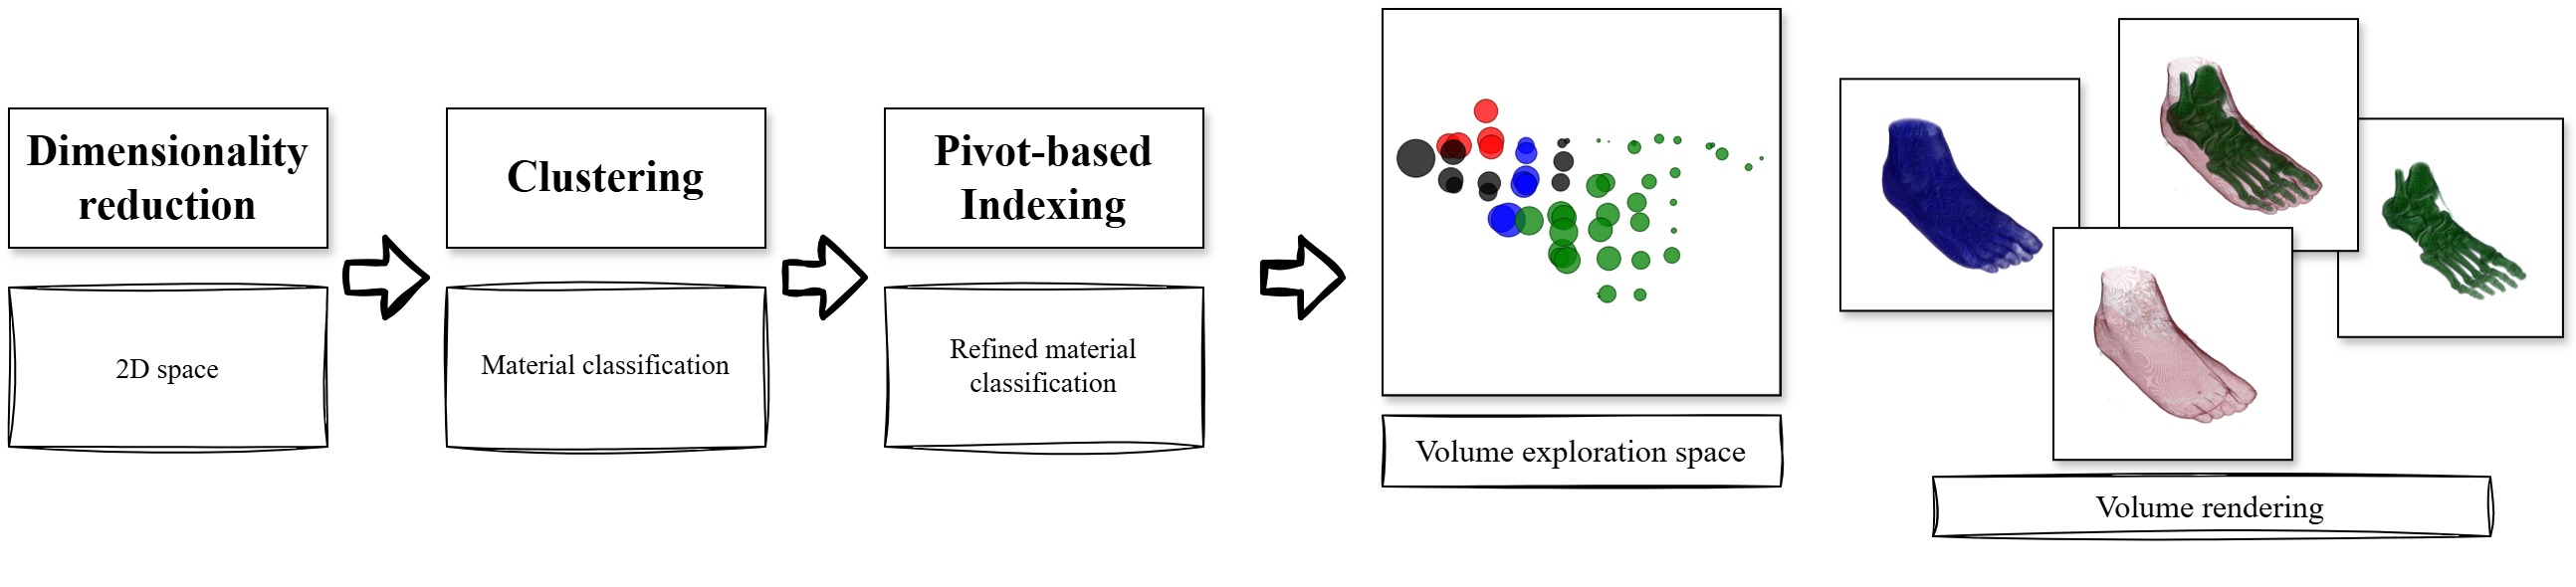
\includegraphics[width=\textwidth]{figs/method-overview.jpg}
\end{figure*}

\subsection{Dimensionality Reduction}
\label{subsect:feature-extraction}

We use FastMap~\cite{faloutsos1995} to project high-dimensional data into 2D while preserving clustering structure. The algorithm finds two distant pivots and projects points onto the line between them.

Let $d$ be the number of attributes and $n$ the number of voxels. The steps are:
\begin{enumerate}
    \item Find two points (pivots) furthest apart.
    \item Project points onto a hyperplane orthogonal to the pivots’ line.
\end{enumerate}

To avoid quadratic complexity, we use the heuristic from~\cite{faloutsos1995} (Algorithm~\ref{alg:pivot-searching-of-fastmap}) which approximates distant pivots.

\begin{algorithm}
    \caption{Pivot searching of FastMap.}
    \label{alg:pivot-searching-of-fastmap}
    \KwIn{$\mathbb{O}$}
    \KwOut{Pivots $O_a$, $O_b$}
    $O_a \gets$ random point $o \in \mathbb{O}$\\
    $O_b \gets$ point $o \in \mathbb{O}$ farthest from $O_a$\\
    $O_a \gets$ point $o \in \mathbb{O}$ farthest from $O_b$
\end{algorithm}

Time complexity is $\mathcal{O}(nk)$ with $k=2$.

\subsection{Clustering}
\label{subsect:clustering}

To simplify classification and highlight details, we use DBSCAN~\cite{ester1996}. Since the original has worst-case $\mathcal{O}(n^2)$ complexity, we adopt a grid-based variant~\cite{gunawan2013} with $\mathcal{O}(n \log n)$ complexity.

Parameters $minPts$ and $\varepsilon$ must be tuned by the user. The algorithm partitions space into a grid, estimates density, identifies core points, expands clusters, assigns border points, and labels noise.

\subsection{Pivot-based indexing}
\label{subsect:pivot-based-indexing}

To reduce scatter plot clutter, we plot only selected pivots within each cluster. Each cluster is subdivided into sub-clusters by assigning points to their nearest pivot (Algorithm~\ref{alg:subclustering-finding}).

\begin{algorithm}
    \caption{Finding sub-clusters within a cluster.}
    \label{alg:subclustering-finding}
    \KwIn{Points $\mathbb{P}$ of cluster $c$}
    \KwIn{Pivots $\mathbb{P}_s$ of cluster $c$}
    \KwOut{Points with sub-cluster assignment}
    \ForEach{$p \in \mathbb{P}$}{
        $p_s \gets$ nearest pivot in $\mathbb{P}_s$ \\
        Assign $p$ to $p_s$'s sub-cluster
    }
\end{algorithm}

We select pivots using Sparse Spatial Selection (SSS)~\cite{pedreira2007}, which adds points as pivots if they are sufficiently distant from existing ones, controlled by a distance factor $\alpha$.

\begin{algorithm}
    \caption{Sparse Spatial Selection.}
    \label{alg:sss}
    \KwIn{Points $\mathbb{P}$}
    \KwOut{Selected pivots $\mathbb{P}_s$}
    $\mathbb{P}_s \gets \{p_1\}$ \\
    \ForEach{$p \in \mathbb{P}$}{
        \If{$\forall p_s \in \mathbb{P}_s, \text{dist}(p, p_s) \geq M\alpha$}{
            $\mathbb{P}_s \gets \mathbb{P}_s \cup \{p\}$
        }
    }
\end{algorithm}

Adjusting $\alpha$ controls the number of pivots: smaller $\alpha$ selects more pivots; values near $1$ select fewer.

